\chapter{2変数函数のグラフ}

\lectureinfo{2015年5月13日 1限}

\section{講評}

最初に採点をしてて思ったことを、ちょっとだけ書いておきます。\vspace{-0.5zw}
\begin{itemize}
\item 全体的に正答率は高かったです。
\item グラフを描く問題は、コンピュータで頑張った人と手書きで頑張った人が半々ぐらいでした。またコンピュータを使った人の中ではMathematicaで描いた人が一番多く、次にgnuplotを使った人が多かったと思います。
\item グラフ$z = xy$を回転する問題や平面で切断したときの断面を考える問題は、正答率が極めて低かったです。$2$変数函数のグラフの回転操作は、まだなじみがなかったのかもしれません。「グラフの平行移動のやり方」と「点の回転のしかた」が分かれば、グラフの回転もできるようになります。落ち着いて復習してみてください。
\end{itemize}\vspace{-2zw}

\section{2変数函数のグラフの切断}

$2$変数函数$z = f(x, y)$のグラフは$3$次元的形状を持つため、$1$変数函数のグラフと比べて理解が難しくなります。それを何とかするための一つの手段として「平面で切断した様子を観察する」という手があります。

前回の内容を思い出しましょう。「$x, y, z$の$1$次方程式が定める図形は平面である」という事実を確認しました。ですからグラフの方程式$z = f(x, y)$と平面の方程式$ax + by + cz + d = 0$を連立すれば、グラフ$z = f(x, y)$の平面$ax + by + cz + d=0$による断面が得られます。特に平面の方程式として分かりやすいもの、たとえば\vspace{-0.5zw}
\begin{itemize}
\item $xy$平面、$yz$平面、$zx$平面のいずれかに平行な平面
\item $z$軸を含む平面
\end{itemize}\vspace{-0.5zw}
を上手く取って来れば、グラフの形状をよく理解できる可能性が高まります。\vspace{-0.5zw}

\subsection{座標軸の張る平面に平行な切断}

\paragraph{等高線}

実数$c$に対し、方程式$z=c$は$z$座標の値が$c$である、$xy$平面と平行な平面を表します。したがって$z = f(x, y)$と連立して$c = f(x, y)$とすれば、平面$z=c$による断面が見えます。この断面のことをグラフの\textbf{等高線}といいます。等高線が把握できれば、$c$の値を動かすことでグラフの形状が把握できます。たとえば$z = \sqrt{x^2+y^2}$と$z = x^2 + y^2$のグラフを、$xy$平面に平行な平面を$z=0$から$z=1$まで$0.1$刻みで動かしてみましょう。

\begin{figure}[h!tbp]
\centering
\subfigure[$z  = \sqrt{x^2+y^2}$]{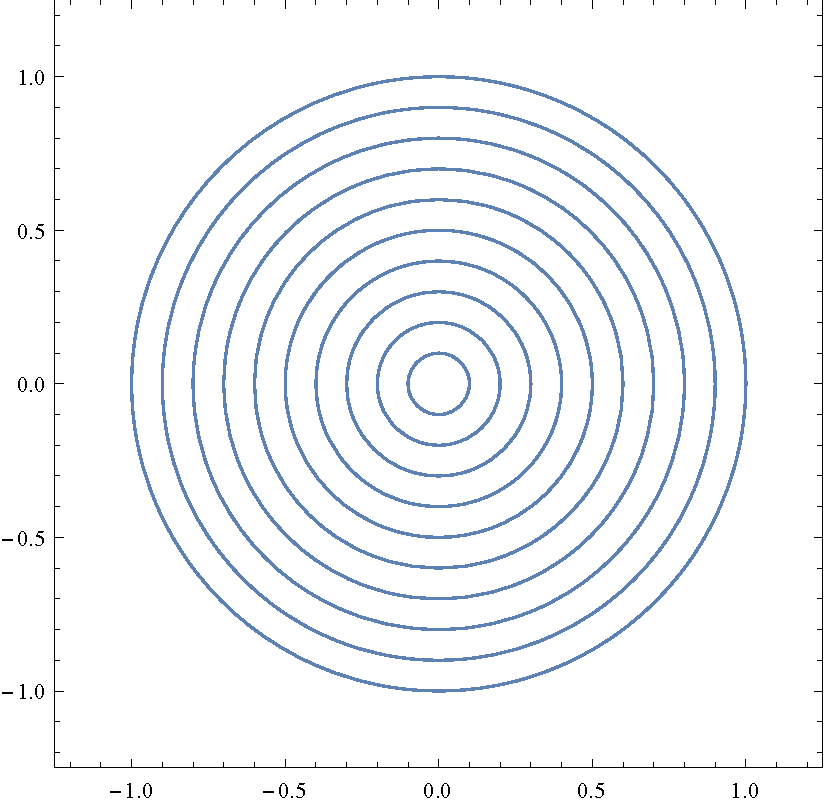
\includegraphics[width = .25\textwidth]{20150513-fig-cone1.pdf}} \quad
\subfigure[$z  = x^2+y^2$]{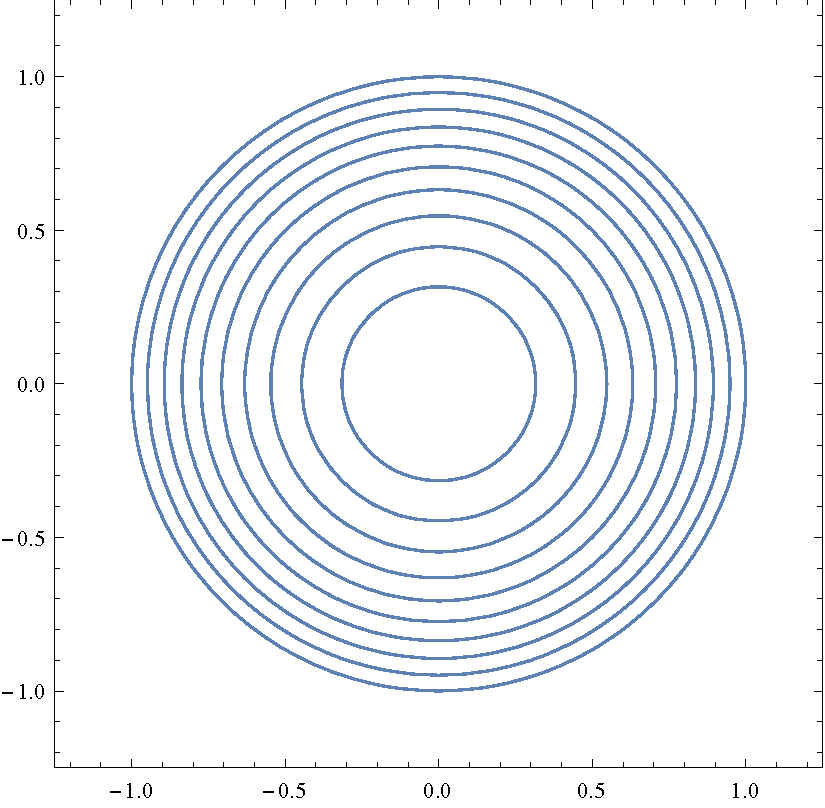
\includegraphics[width = .25\textwidth]{20150513-fig-elliptic-paraboloid1.pdf}}
\end{figure}

この図から明らかに、どちらのグラフも$z$軸回りの回転対称性を持つと分かります。また等高線の密度から、$z = \sqrt{x^2 + y^2}$では高さが一定の間隔で増し、$z = x^2 + y^2$では急激に高さが増していく感じがします。ですがどの程度増えるのかは、この図だけでははっきりしません。詳しい情報を得るためには、他の平面での切断面などが必要です。

\paragraph{$x$軸や$y$軸に垂直な平面での切断}

全く同様に平面$x = c$あるいは$y = c$ ($c\in\mathbb{R}$は定数) を使うことで、それぞれ$x$軸と$y$軸に垂直な平面でグラフを切断できます。

さっきの$z = \sqrt{x^2+y^2}$と$z = x^2 + y^2$で試してみましょう。まずは$x=0$とおくと、式はそれぞれ$z = \sqrt{y^2} = |y|$, $z = y^2$となります。これらが$yz$平面による断面です。そのグラフは次の通りです。

\begin{figure}[h!tbp]
\centering
\subfigure[$z  = |y|$]{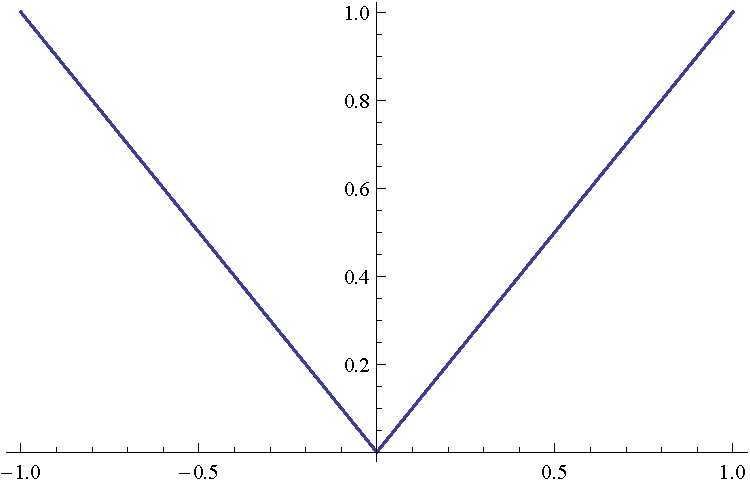
\includegraphics[width = .3\textwidth]{20150513-fig-cone2.pdf}} \quad
\subfigure[$z  = y^2$]{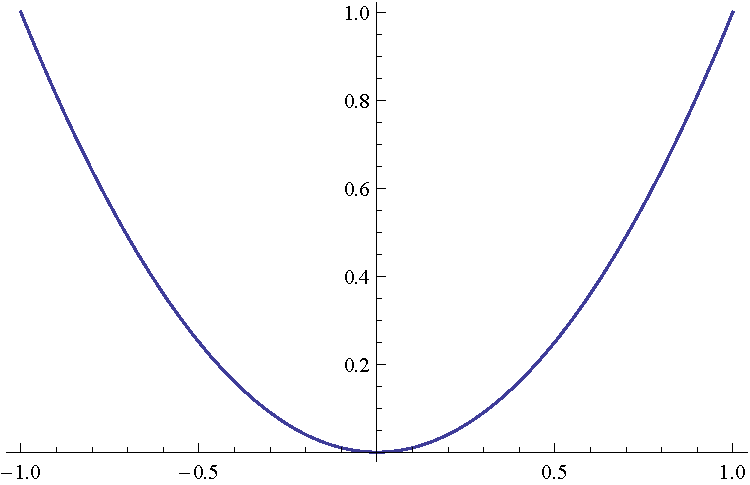
\includegraphics[width = .3\textwidth]{20150513-fig-elliptic-paraboloid2.pdf}}
\end{figure}

あとは$z$軸回りの回転対称性があるので、このグラフを$z$軸回りにぐるっと一周回転させれば求めるグラフの正体が分かります。$z = \sqrt{x^2 + y^2}$は円錐、$z = x^2 + y^2$は回転放物面です。

\begin{figure}[h!tbp]
\centering
\subfigure[$z  = \sqrt{x^2 + y^2}$]{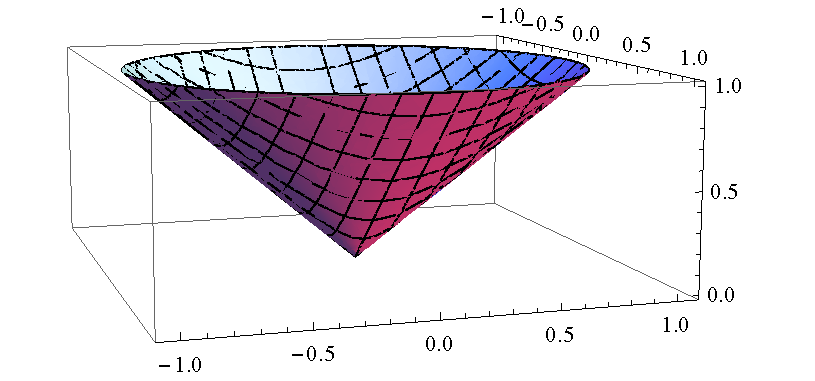
\includegraphics[width = .4\textwidth]{20150513-fig-cone3.pdf}} \quad
\subfigure[$z  = x^2 + y^2$]{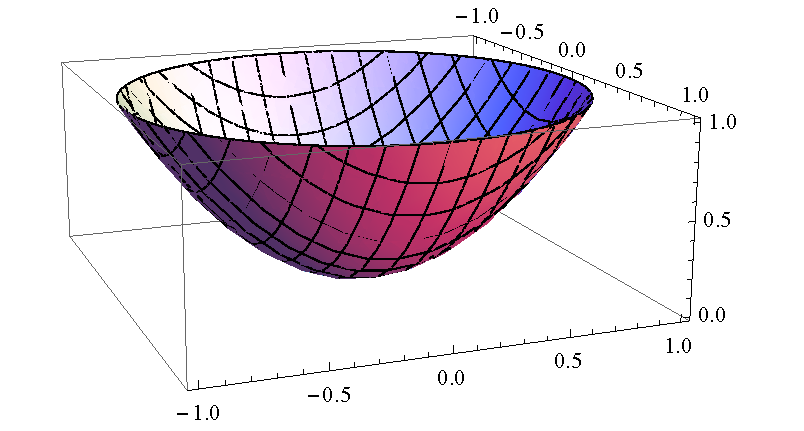
\includegraphics[width = .4\textwidth]{20150513-fig-elliptic-paraboloid3.pdf}}
\end{figure}

また$x$, $y$軸に垂直な平面に関するグラフの切断は、$2$変数函数$f(x, y)$を$x, y$の順に積分するときに役立ちます。特に体積の計算をするときは、まず真っ先にこれらの切断を考えるでしょう。ほとんどの人が大学入試の勉強でやったことがあるはずです。

\subsection{$z$軸を含む平面に関する切断}

続いて平面の方程式のうち、$ax + by = 0$の形のものを考えます。これの法ベクトルは${}^t\!(a, b, 0)$で、$z$軸の方向ベクトル${}^t\!(0, 0, 1)$と直交します。さらに平面$ax + by = 0$は原点を通るので、この平面は$z$軸を含むことが分かりました。したがって方程式$z = f(x, y)$で$ax + by = 0$を連立して$x$ないし$y$を消去すれば、$z$軸を含む平面でどういう形をしているか分かります。この式で$b=0$や$a=0$とした場合は、先ほどの$x$, $y$軸に垂直な平面による切断と一致します。

たとえば方程式$z=xy$のグラフを考えましょう。次のように変形してみます。
\begin{align*}
z = xy = \frac{(x+y)^2 - (x-y)^2}{4}
\end{align*}

この式に$x=y$を代入すると$z=x^2$、$x=-y$を代入すると$-x^2$になります。したがって平面$x=y$での断面は上向きの放物線、それに直交する平面$x=-y$での断面は下向きの放物線となります。ただし、\textbf{この放物線がそのまま$y=\pm x^2$にはならない}ことに気を付けてください。直線$y = x$上で原点からの距離が$1$である点のうち、座標が正のものは$(1/\sqrt{2}, 1/\sqrt{2})$です。ですから$xy$平面の直線$y=\pm x$に$x$軸や$y$軸と同じ目盛りを刻むには、点$(1/\sqrt{2},1/\sqrt{2})$を基準に取らなければいけません。そうすると$(x,y) = (t/\sqrt{2},\pm t/\sqrt{2})$のとき$xy = \pm t^2/2$となりますから、$z = xy$の平面$x = \pm y$による断面の放物線は$y = \pm x^2/2$と合同になります。

一方で等高線は$xy = c$という反比例の式で定まるので、双曲線または$2$直線になります。これを踏まえ、次の平面図を見てください。実線が$z\geq 0$の部分、点線が$z<0$の部分の等高線です。そして斜めの実線と点線がそれぞれ平面$x=y$と$x=-y$に対応し、これらで切断した断面がそれぞれ上向きと下向きの放物線になるわけです。

\begin{figure}[h!tbp]
\centering
\subfigure[$z = xy$を上から見た図]{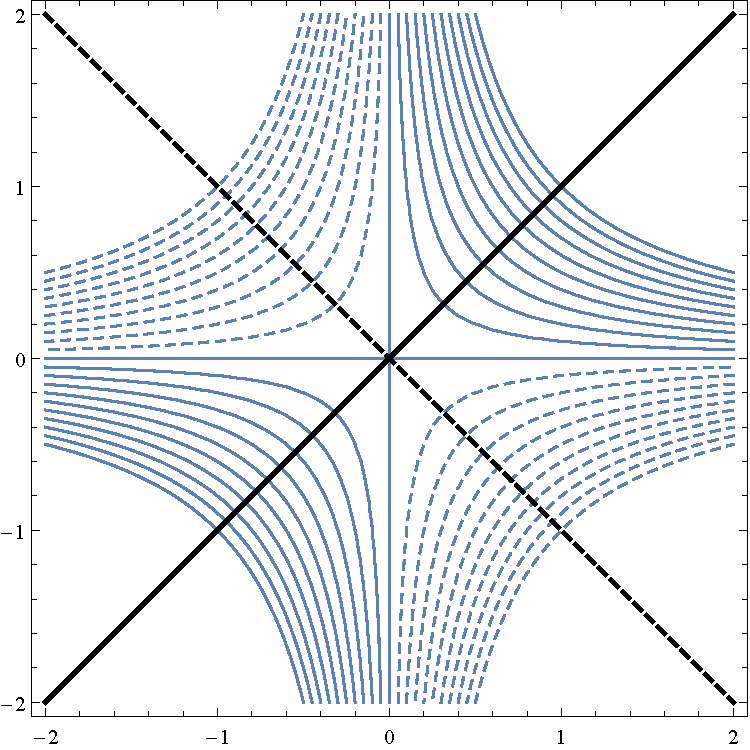
\includegraphics[width = .3\textwidth]{20150513-fig-hyperbolic-paraboloid1.pdf}} \quad
\subfigure[$z = xy$を俯瞰した図]{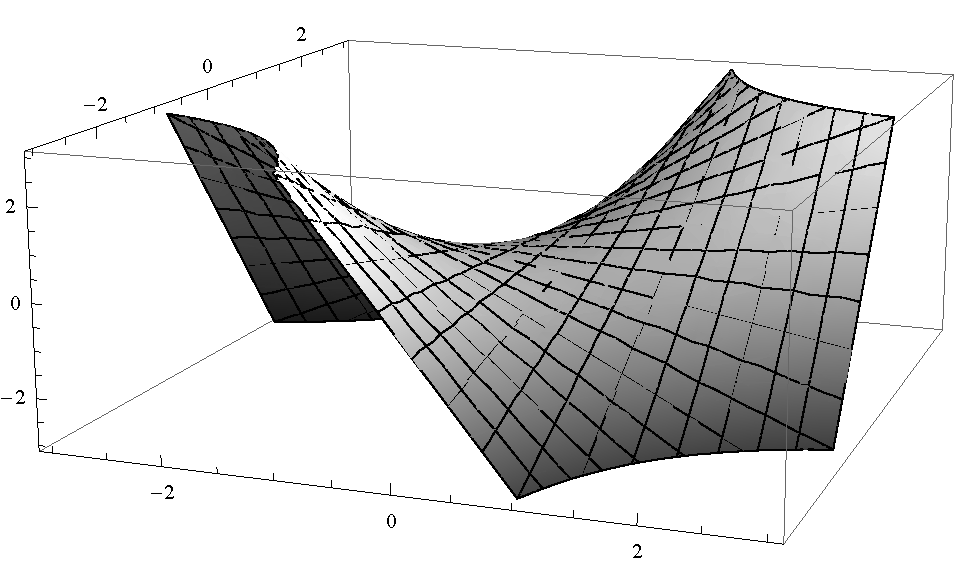
\includegraphics[width = .45\textwidth]{20150513-fig-hyperbolic-paraboloid2.pdf}}
\end{figure}

そして右の図は、曲面$z = xy$を俯瞰した図です。このグラフは双曲放物面と呼ばれます\footnote{テキストに「双曲$2$次形式」とも書いてありますが、これはどちらかというと$x^2-y^2-z=0$という「式の形」を表す言葉です。岩波書店から出ている『数学辞典 第$4$版』を引くと347 Aの項に「双曲放物面」と書いてあるので、その呼び名を使いました。また、このグラフで原点は「接平面が$xy$平面と平行であるが、極大でも極小でもない」という意味で\textbf{鞍点}と呼ばれます。ただしこれは一般名詞であって、グラフを固有名詞的に「馬の鞍」と呼ぶわけではありません。気を付けてください。}。立体的な図を見て等高線が双曲線になること、それから断面に放物線が現れることを納得してください\footnote{PDFファイルの原本 \url{https://github.com/HideakiHosaka/2015_linear_algebra/raw/master/2015linear_algebra.pdf} も必要に応じて見てみてください。カラーな上に拡大可能なので、印刷版より図が綺麗なはずです。}。

\begin{figure}[h!tbp]
\centering
\subfigure[$z = xy$の平面$x = y$による断面]{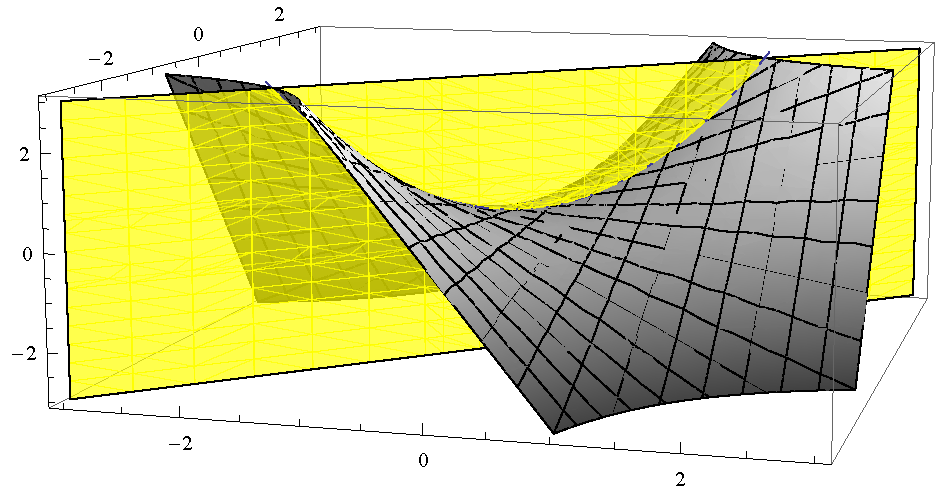
\includegraphics[width = .5\textwidth]{20150513-fig-hyperbolic-paraboloid3.pdf}} \quad
\subfigure[$z = xy$の平面$x = -y$による断面]{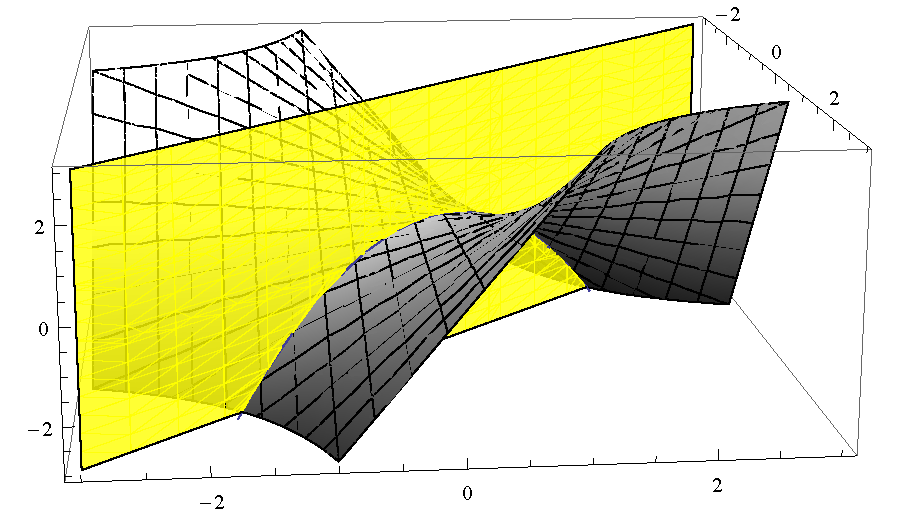
\includegraphics[width = .45\textwidth]{20150513-fig-hyperbolic-paraboloid4.pdf}}
\end{figure}

\section{座標変換とグラフの移動}

$2$変数函数のグラフを理解する別の手段として、グラフの移動を考えます。$1$変数の場合、この手法の最も典型的な例は平方完成です。$2$次函数を平方完成をすると、その$2$次函数が「放物線$y=ax^2$をどうやって動かして作られたか」が分かり、それによってグラフの形状がはっきり分かるのでした。そこで$2$変数函数についても、グラフを動かしましょう。$2$変数の場合は平行移動だけでなく回転移動もできますから、回転移動の方法についても調べます。

また$2$変数以上の函数だと、グラフを移動する以外にも「座標を取り換える」という操作ができます。$1$変数函数だと、せいぜい値域の目盛りを対数軸にして対数プロットをすることがあるくらいで、定義域の目盛りを変えることはありませんでした。ところが$2$変数函数だと、座標の取り換えが極めて有効なケースが出てきます。

\subsection{円柱座標}
平面上の極座標は、$(x,y) = (r\cos\theta, r\sin\theta)$ という式で定義されていました。そこで直交座標$(x,y,z)$のうち$x, y$だけを極座標で置き換えることで$(r,\theta,z)$という座標系が定まります。これを円柱座標といいます\footnote{$3$次元の極座標$(r,\theta,\varphi)$とは別物です。}。

$z=f(x,y)$の式の中にあからさまに$x^2+y^2$が出てくるなどする場合は、円柱座標が役立ちます。たとえばさっきの$z=\sqrt{x^2+y^2}$というグラフを円柱座標で考えてみると、$x^2+y^2=r^2$より$z=\sqrt{r^2}=|r|$となります。だから$z$の値は$\theta$に依存せず、グラフが$z$軸回りの任意の角度に対する回転対称性を持つことが分かります。そして$z$軸を含む平面でグラフを切断すれば、$z=|r|$という絶対値のグラフが現れます。これを回転させることで、元々のグラフは円錐を表していたことが再び分かります。このように$z$軸回りの回転対称性を持つグラフは、円柱座標を使う事ですっきりと理解できます。

$z=x^2+y^2$のグラフでも状況は同じです。こっちでは$z=r^2$となるのでやはり回転対称性を持ち、さらに$z$軸を含む平面での断面は放物線になります。よって放物線を軸に回転させて、元のグラフが回転放物面だと分かります。

\subsection{平行移動}
函数$y=f(x)$のグラフを右に$a$だけ平行移動すると、式は$y=f(x-a)$に変化します。右に$a$ずらすときに$f$の中に$x-a$が入るのでたまに勘違いしそうになりますが、そういうときは$x=0$等で検証してみましょう。平行移動後に$x=0$の位置\textbf{に写ってくる}のは、元々左に$a$だけ移動したところにある$x=-a$の位置の点です。だから平行移動後のグラフで$x=0$における値は$f(-a)$となります。

多変数函数でも全く事情は同じです。$z=f(x,y)$のグラフを$x$軸正の方向に$a$, $y$軸正の方向に$b$だけ平行移動させるとき、平行移動で点$(x, y)$\textbf{に写ってくる}点は$(x-a, y-b)$です。よって平行移動後のグラフは$z=f(x-a,y-b)$になります。

\subsection{回転}

$1$変数のグラフは変数が$x$しかないので、グラフの移動といっても平行移動くらいしかすることがありません。ですが$2$変数のグラフになると、座標の回転ができるようになります。原点中心の回転を調べてみましょう。平行移動のときと同じく、見るべきは「回転移動でどの点がどこに写るか」ではなく「どの点が\textbf{どこから写ってくるか}」です\footnote{後々線型代数の授業で座標変換を考えるときも、これと似たような状況が現れます。}。

複素平面上で原点中心の角度$\theta$回転は、$e^{i\theta}$の掛け算で与えられるのでした。これと$e^{i\theta}e^{-i\theta}(x+iy)=x+iy$より、$\theta$回転で点$(x,y)$\textbf{に写ってくる}点は$e^{-i\theta}(x+iy) = \bigl((\cos\theta) x + (\sin\theta)y \bigr) + i\bigl(-(\sin\theta) x + (\cos\theta) y\bigr)$です。したがって$f(x,y)$を原点中心に$\theta$回転させて得られる函数は、$f(x,y)$の中に今の座標を代入して得られる$f\bigl((\cos\theta) x + (\sin\theta)y, -(\sin\theta) x + (\cos\theta) y\bigr)$です。

% 群の函数への作用

さっきの$z = xy$のグラフは、回転を使うとよく理解できます。$xy$座標系を正の向きに$\pi/4$だけ回転させて$uv$座標系を作ります。すると導いた回転の公式で$\theta=\pi/4$を代入することで、$uv$座標系での点$(u,v)$は$xy$座標系で$\bigl((u+v)/\sqrt{2},(u-v)/\sqrt{2}\bigr)$に化けます。したがって$z = xy$は$uv$座標系で$z = (u^2-v^2)/2$です。こうすれば曲面$z = xy$と$z = x^2-y^2$が回転と縦方向の拡大・縮小で写り合うことが分かります。既に確認した通りですね。ちなみに$z = (u^2-v^2)/2$に直してしまえば、どんな定数$c\in\mathbb{R}$に対しても、平面$u = c$での断面が放物線$z = -v^2 /2$と同じ形だと分かります。実際$z = -v^2/2 + c^2/2$は、放物線$-v^2/2$を上下方向に平行移動したものです。これを$xy$座標系で見れば、平面$y = -x + c$ ($c\in\mathbb{R}$)による断面となります。

また今は$z$軸を中心とする回転を調べましたが、軸が$z$軸と平行である限り、どこであっても回転の計算はできます。既に僕たちはグラフの平行移動の仕方を知っていますから、回転軸が一旦$z$軸と重なるように平行移動し、$z$軸回りの回転をして、さらに最初の平行移動とは逆向きの平行移動をすればOKです。

\section{曲面上の運動と接ベクトル}

\subsection{曲面に沿う曲線と接ベクトル}

$2$変数函数$z=f(x,y)$と平面$\mathbb{R}^2$内の曲線$\gamma$を考えます。各$t\in\mathbb{R}$に対して平面$\mathbb{R}^2$上の点$\gamma(t)\in\mathbb{R}^2$が定まるから、$\gamma(t) = \bigl(x(t), y(t)\bigr)$と書けます。そこで$\gamma(t)$の座標を$z = f(x, y)$に代入する\footnote{写像の言葉で言うなら、曲線を$\gamma\colon\mathbb{R}\rightarrow\mathbb{R}^2$という写像と思い、$2$変数函数$f\colon\mathbb{R}^2\rightarrow\mathbb{R}$の合成$f\circ\gamma$を考えています。}と、$f\bigl(x(t), y(t)\bigr)$は点$\gamma(t)$における$f$の値を表します。こうしてしまえば$f\bigl(x(t), y(t)\bigr)$は$t$の函数ですから、微分することができます。まだ証明していませんが、実は$f\bigl(x(t), y(t)\bigr)$の$t$における微分は$f$と$\gamma'(t) := \bigl(x'(t), y'(t)\bigr)$だけで決まります\footnote{合成函数の微分さえできれば良いのですが、それは多変数の場合「連鎖律」と呼ばれ、少しだけ計算が複雑になります。}。そこで$f\bigl(x(t), y(t)\bigr)$の微分を、$\gamma'(t)$方向の\textbf{方向微分}と言います。$t$を時刻、$\gamma$を点の運動だと思えば、$\gamma'(t)$は時刻$t$における速度ベクトルです。直感的に言うと$f\bigl(\gamma(t)\bigr)$の微分は「$\gamma'(t)$方向に少し動くとどれだけ$f$が変化するか」を表す量ですから、方向微分という言葉がしっくりくるのではないでしょうか。

また$\tilde{\gamma}(t):=\bigl(x(t), y(t), f(x(t), y(t))\bigr)$と置くと、$\tilde{\gamma}(t)$は常に曲面$z = f(x,y)$上の点を表します。したがって$t$を動かすことで、曲面$z = f(x, y)$に沿う曲線が得られます。そこで曲線$\tilde{\gamma}$の座標を$t$で微分すると、$\tilde{\gamma}$の接ベクトルができ、それが曲面$z = f(x, y)$の接ベクトルにもなります。このようにして、曲面の接ベクトルが得られます。

\subsection{偏導函数と接平面}

今の方向微分の話で、特に$\gamma(t) = (a+t, b)$あるいは$\gamma(t) = (a, b+t)$の場合を考えます。つまり$\gamma$は$x$軸や$y$軸の方向を向いた直線の上を、速度$1$で進みます。このとき$f\bigl(\gamma(t)\bigr)$を$t=0$で微分した値を、それぞれ点$(a, b)$における$x$方向、$y$方向の\textbf{偏微分係数}といいます。すなわち
\[
\frac{\partial f}{\partial x}(a, b) := \frac{d}{dt}f(a+t, b)\Bigr|_{t=0}, \quad \frac{\partial f}{\partial y}(a, b) := \frac{d}{dt}f(a, b+t)\Bigr|_{t=0}
\]
です。新しい記号が出てきましたが、計算自体は難しくありません。$x$での偏微分は「$y$を定数と思って、$x$の函数として微分する」というだけです。また$1$変数の場合、微分係数は接線の傾きでした。だから$x$での偏微分係数は、点$(a,b)$における曲面$z = f(x, y)$の$x$軸方向の勾配を表します。

これを知っていると、$2$変数函数のグラフ$z = f(x, y)$の接平面が求められます。$\tilde{\gamma}$の微分が曲面$z = f(x,y)$の接ベクトルでした。その式に$x$方向の偏微分と$y$方向の偏微分を代入すると
\[
\biggl(1, 0, \frac{\partial f}{\partial x}(a, b)\biggr),\quad \biggl(0, 1, \frac{\partial f}{\partial y}(a, b)\biggr)
\]
が曲面$z = f(x,y)$の点$(a, b)$における接ベクトルだと分かります。これらのベクトルは$1$次独立ですから、点$(a, b)$における接平面はこれら$2$本のベクトルによって張られます。したがって外積を使って、接平面の法ベクトルが
\[
\biggl(\frac{\partial f}{\partial x}(a, b), \frac{\partial f}{\partial y}(a, b), -1\biggr)
\]
と分かります。これで接平面の方程式における$x, y, z$の係数が決まりました。あとは接平面が点$\bigl(a, b, f(a,b)\bigr)$を通るよう調整すれば、接平面の方程式
\[
\frac{\partial f}{\partial x}(a, b) (x-a) + \frac{\partial f}{\partial y}(a, b) (y-b) - \bigl( z - f(a,b)\bigr) = 0
\]
が求まります。

\section{解答など}

\subsection{穴埋め問題の解答}

既に一通りの問題を解説していますが、穴埋め問題の解答だけをもう一度まとめておきます。

\begin{tabular}{c@{\hspace{0.1zw}}l@{\hspace{1zw}}c@{\hspace{0.1zw}}l@{\hspace{1zw}}c@{\hspace{0.1zw}}l@{\hspace{1zw}}c@{\hspace{0.1zw}}l@{\hspace{1zw}}c@{\hspace{0.1zw}}l@{\hspace{1zw}}c@{\hspace{0.1zw}}l@{\hspace{1zw}}c@{\hspace{0.1zw}}l@{\hspace{1zw}}c@{\hspace{0.1zw}}l@{\hspace{1zw}}}
(1) & 平面 & (2) & 双曲放物面 & (3) & $z$軸 & (4) & 回転対称性 & (5) & 円錐 & (6) & 回転放物面 & (7) & $a$ & (8) & $b$ \\
(9) & $\sqrt{c}$ & (10) & $2xy$ & (11) & 双曲放物面 & (12) & 双曲線 & (13) & $a$ & (14) & $b$ & (15) & $1/2$ & (16) & $-1/2$ \\
\end{tabular}

\subsection{グラフ}
$z = xy$のグラフは既に描きました。$z = x \sin y$と$z = \sin x\sin y$のグラフは次の通りです。グラフの雰囲気が分かるよう、問題より少し範囲を広げて描画しています。
\begin{figure}[h!tbp]
\centering
\subfigure[$z  = x \sin y$]{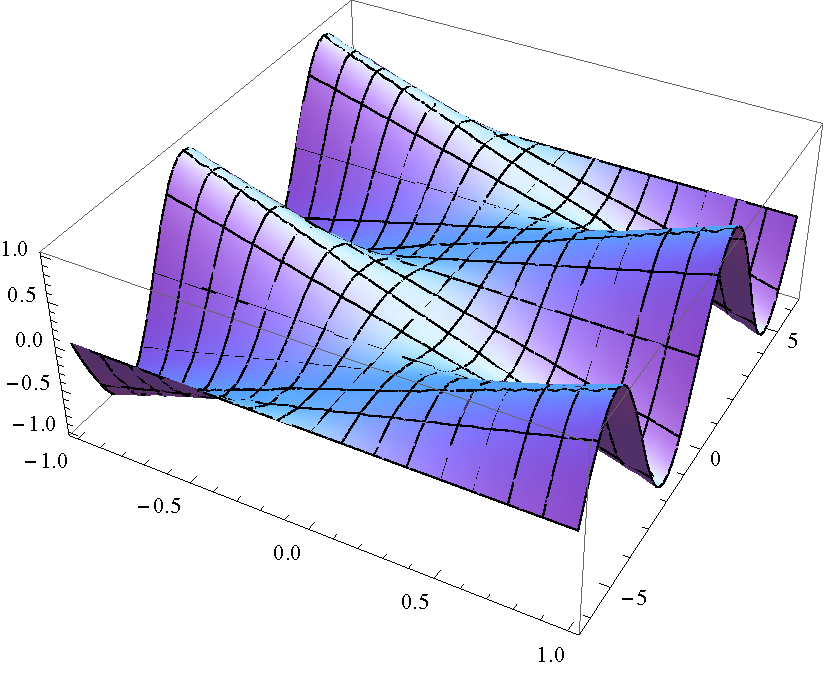
\includegraphics[width = .4\textwidth]{20150513-fig-problem-b.pdf}} \quad
\subfigure[$z  = \sin x \sin y$]{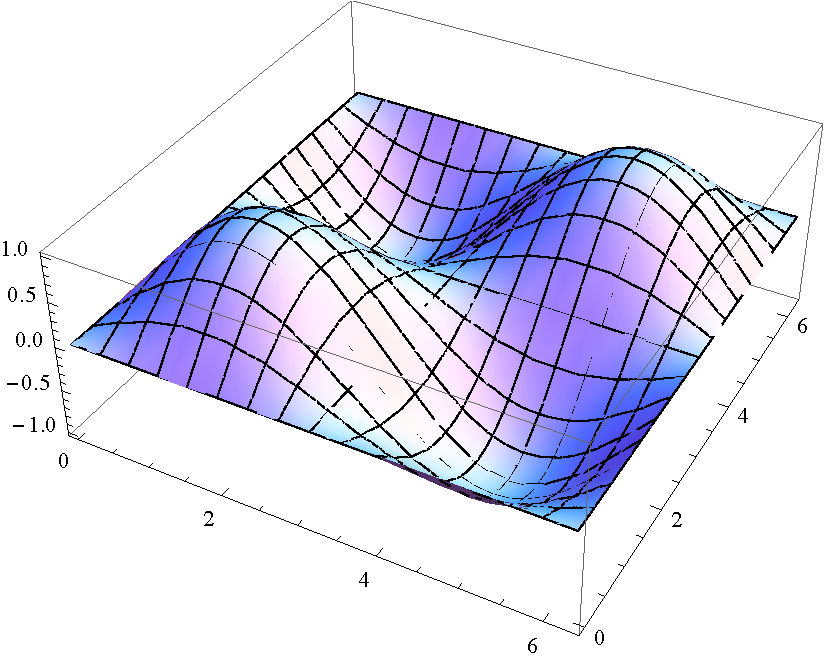
\includegraphics[width = .4\textwidth]{20150513-fig-problem-c.pdf}} \quad
\end{figure}

ちなみに、これらのグラフはMathematicaを使って描いています。Mathematicaの使い方については、たとえば「はいぱーワークブック」の29章\footnote{\url{http://hwb.ecc.u-tokyo.ac.jp/current/applications/mathematica/}}や、そこに紹介されている参考文献などを読んでください。

